\documentclass{article}
\usepackage{floatflt,epsfig}
\usepackage[utf8]{inputenc}
\usepackage[T1]{fontenc}
\usepackage{lipsum}
\usepackage{graphicx}
\usepackage{float}
\usepackage{amsmath}
\usepackage[margin=1in]{geometry}
\usepackage{titlesec}
\usepackage{listings}
\usepackage{xcolor}
\usepackage{hyperref}
\usepackage{subfigure}

\hypersetup{
    pdfborder = {0 0 0},
}

\lstdefinelanguage{Java}{
    keywords={abstract,assert,boolean,break,byte,case,catch,char,class,const,continue,default,do,double,else,enum,extends,false,final,finally,float,for,goto,if,implements,import,instanceof,int,interface,long,native,new,null,package,private,protected,public,return,short,static,strictfp,super,switch,synchronized,this,throw,throws,transient,true,try,void,volatile,while},
    morekeywords={[2]System,out},
    morecomment=[l]{//},
    morecomment=[s]{/*}{*/},
    morestring=[b]",
    basicstyle=\small\ttfamily,
    keywordstyle=\color{blue}\bfseries,
    keywordstyle={[2]\color{orange}\bfseries},
    commentstyle=\color{green!70!black},
    stringstyle=\color{red},
    showstringspaces=false,
    tabsize=2,
    breaklines=true,
    breakatwhitespace=true,
    frame=single,
    captionpos=b
}

\titleformat{\section}
{\LARGE\bfseries}{\thesection}{1em}{}

\titleformat{\subsection}
{\Large\bfseries}{\thesection}{1em}{}

\begin{document}
    \pagestyle{empty}
    \begin{titlepage}
        \begin{center}
        {{\Large{\textsc{Alma Mater Studiorum - Università di Bologna}}}}
            \rule[0.1cm]{\textwidth}{0.1px}
            \rule[0.5cm]{\textwidth}{0.6px}\\
            {\large{SCUOLA DI SCIENZE \\ Corso di Laurea in Informatica per il Management}}
        \end{center}

        \vspace{90px}

        \begin{center}
            \LARGE Personal Physical Tracker
        \end{center}

        \vspace{100px}
        \par
        \noindent
        \hfill
        \begin{minipage}[t]{0.4\textwidth}\raggedleft
        {\fontsize{12}{13}{}\
            \fontsize{12}{13}{\\ Canghiari Matteo \\ Matricola 1032059 \\ matteo.canghiari@studio.unibo.it}}
        \end{minipage}

        \vspace*{140px}

        \begin{center}
            \large{Laboratorio di Applicazioni Mobili}\\
            \large{Anno Accademico 2023/2024}
        \end{center}
    \end{titlepage}

    \newpage
    \subsection*{Introduzione}
    \large

    \textbf{Personal Physical Tracker} è un'applicazione nativa Android, che permette di registrare le attività motorie quotidiane che possano essere compiute durante la giornata,
    contraddistinte in \textbf{camminata}, \textbf{spostamenti tramite veicoli}, \textbf{attività sedentarie} e \textbf{corsa}.
    L'obiettivo dell'applicazione consiste nello sviluppo di un sistema software in grado di poter memorizzare dati riferiti alle attività compiute, favorendo un'interfaccia 
    grafica semplice e di facile utilizzo, da cui sia possibile osservare attivamente le informazioni manipolate e rappresentate.
    L'insieme delle funzionalità saranno successivamente approfondite nella sezione \textbf{Feature}, tuttavia è possibile anticipare il contenuto che contraddistingue il progetto
    proposto. \vspace*{7pt}\\
    Ad un primo avvio l'utente visualizza la schermata per la registrazione, in cui può effettuare il \textit{Sign In} qualora dovesse essere un nuovo iscritto, oppure il 
    \textit{Login} in caso sia già registrato; infatti, è richiesta totale univocità pur di garantire la persistenza dei dati. 
    Proseguendo, viene mostrato il layout principale dell'applicazione, responsabile dell'avvicendamento dei molteplici \textit{Fragment} ospitati al suo interno, composto da una
    \textit{Navigation Bottom Bar} e da un \textit{Drawer}. Mediante la \textit{Navigation Bar}, l'utente possiede la facoltà di \textbf{registrare manualmente} nuove attività, 
    accedere al \textbf{pannello di controllo}, visualizzare i propri \textbf{progressi}, osservare le \textbf{geofence di interesse}, \textbf{pianificare} le proprie attività e,
    infine, visualizzare le attività condivise da altri iscritti nella sezione \textbf{Group}. \vspace{7pt}\\
    Di seguito sono brevemente descritte alcune scelte implementative e strumenti utilizzati durante lo sviluppo: per il versionamento del codice è stato utilizzato \textbf{Git},
    con repository accessibile su \textbf{GitHub}, mentre l'applicativo è stato sviluppato tramite il linguaggio di programmazione \textbf{Kotlin}. Il progetto si 
    compone di quattro punti cardine per il corretto funzionamento, suddivisi in:
    \begin{itemize}
        \renewcommand{\labelitemi}{-}
        \item Design pattern architetturale \textbf{MVVM}, utilizzato per separare il \textbf{Model}, ovvero il contenitore di dati, e la sezione attiva, la \textbf{View}. In questo modo si garantisce la separazione dei componenti, riducendo l'accoppiamento e le dipendenze funzionali, che potrebbero causare massicci problemi in seguito a piccole modifiche
        \item \textbf{Jetpack Compose}, un toolkit moderno utilizzato per velocizzare l'implementazione della \textit{User Interface} in determinate circostanze; dato il suo approccio dichiarativo e di facile intuizione ha permesso di incrementare e migliorare l'interattività dell'applicazione per specifiche componenti
        \item \textbf{Room}, utilizzato per garantire la persistenza dei dati all'interno di un \textit{Database Relazionale Locale}
        \item \textbf{Supabase}, utilizzato per garantire un'ulteriore livello di persistenza dei dati, affinchè il \textit{Database Locale} mantenga al suo interno un unico utente come riferimento, delegando al \textit{Real Time Database} il compito di salvaguardare l'insieme di tutti i dati degli utenti iscritti
        \item \textbf{Amazon S3}, utilizzato per salvare in cloud i dati degli utenti tramite un \textbf{dump} del Database, consentendo la condivisione dell'informazioni memorizzate
    \end{itemize}

    \newpage
    \subsection*{Features}
    \large

    \textit{Registrazione} \vspace*{7pt}\\
    All'avvio dell'applicazione è richiesta la registrazione. Come già ribadito, è necessario che le credenziali siano univoche, per garantire la persistenza dei dati.
    Accettate e registrate quest'ultime, è richiesto il permesso di \textbf{Post Notification}, garantendo l'opportunità di inviare delle notifiche al dispositivo; in caso dovesse essere negato, è concesso ugualmente l'accesso. Tale feature richiede una \textit{connessione ad Internet} stabile, per controllare l'unicità delle credenziali
    all'interno di \textit{Supabase}.
    \begin{center}
        \begin{figure}[H]
            \centering
            \subfigure[Login Activity]{
                \fbox{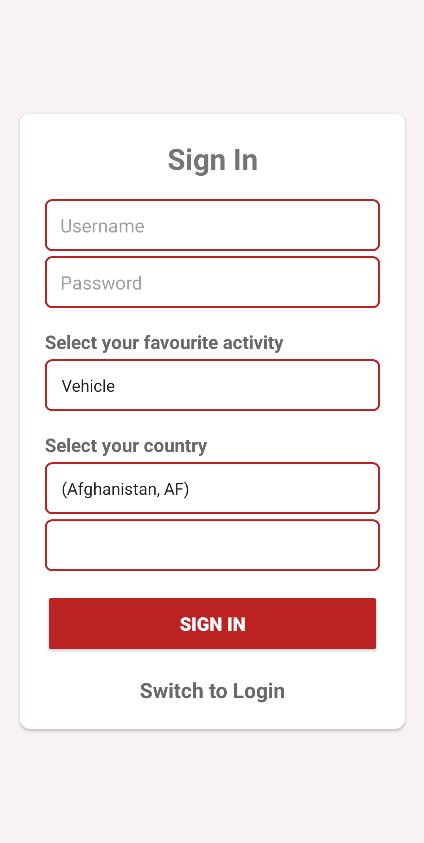
\includegraphics[width=0.35\textwidth]{img1.png}}
            }
            \subfigure[Sign In Activity]{
                \fbox{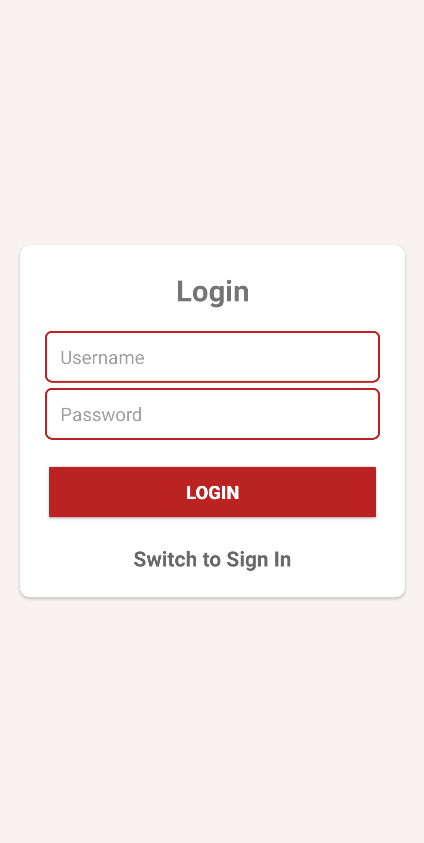
\includegraphics[width=0.35\textwidth]{img2.png}}
            }
        \end{figure}
    \end{center}
    \textit{Dashboard}  \vspace*{7pt}\\
    Successivamente all'autenticazione, il primo layout presentato riguarda la sezione personale dell'utente. Mediante un \textit{Tab Layout}, è possibile osservare i \textit{progressi}
    ottenuti durante la registrazione delle attività motorie e le \textit{transizioni} verificatesi durante lo stazionamento all'interno delle \textit{Geofence}.
    La \textit{Progress Page} possiede una \textit{View} focalizzata sulla descrizione delle attività compiute attraverso l'ausilio di \textbf{grafici}, mentre la 
    \textit{Geofence Page} evidenzia le \textbf{transizioni} avvenute durante un determinato arco temporale.
    \begin{center}
        \begin{figure}[H]
            \centering
            \subfigure[Page Progress]{
                \fbox{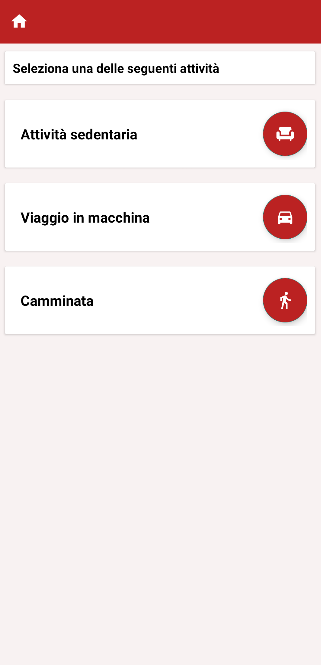
\includegraphics[width=0.35\textwidth]{img3.png}}
            }
            \subfigure[Page Geofence]{
                \fbox{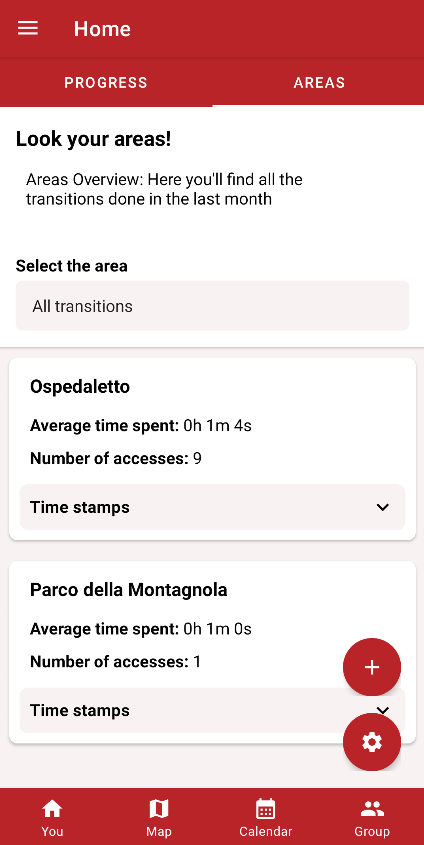
\includegraphics[width=0.35\textwidth]{img4.png}}
            }
        \end{figure}
    \end{center}
    Inoltre, entrambi i \textit{Fragment} ospitano due \textit{Floating Button}; rispettivamente, il primo consente di \textit{registrare manualmente} nuove attività,
    mentre il secondo permette l'accesso al \textit{pannello di controllo}, in cui l'utente può selezionare le proprie preferenze, abilitando oppure disabilitando le funzionalità disponibili. \vspace*{7pt}\\
    \textit{Mappa} \vspace*{7pt}\\
    La \textit{View} contiene una \textbf{mappa} all'interno di un \textit{MapView}. L'utente può inserire, visualizzare ed eliminare le \textit{aree geografiche di interesse};
    una zona di interesse è l'area compresa nel raggio di \{150, 200, 250\} metri, rispetto alle coordinate geografiche che definiscono il centro della circonferenza, varcata
    la soglia di una di esse il dispositivo riceve una notifica personalizzata. 
    Premendo su uno dei molteplici \textit{marker} a disposizione, è mostrato un \textit{Dialog} contenente le informazioni principali della località, tra cui, il nome, la provincia
    e l'indirizzo. 
    \begin{center}
        \begin{figure}[H]
            \centering
            \subfigure[Map Fragment]{
                \fbox{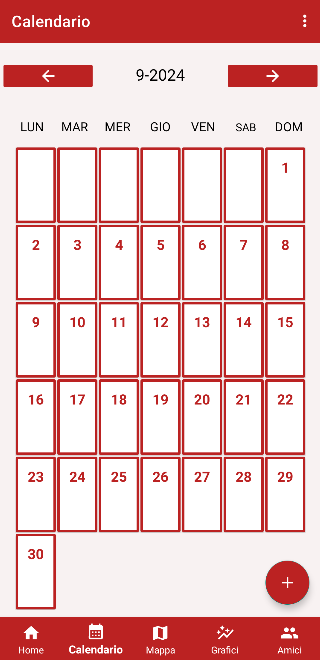
\includegraphics[width=0.35\textwidth]{img5.png}}
            }
            \subfigure[Marker Dialog]{
                \fbox{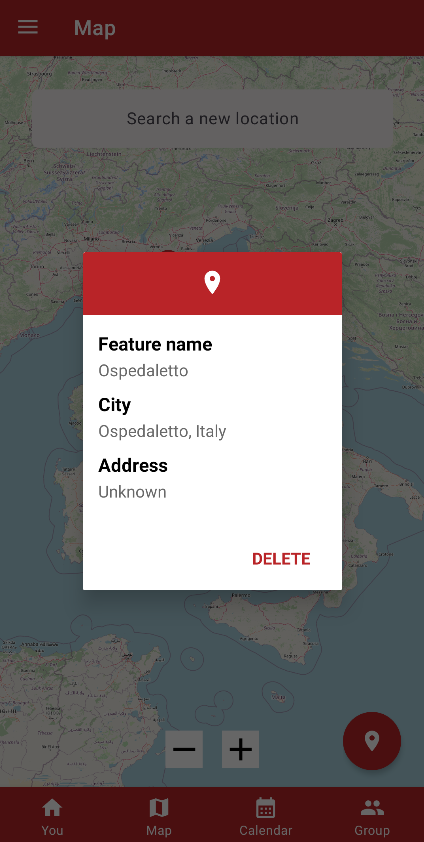
\includegraphics[width=0.35\textwidth]{img6.png}}
            }
        \end{figure}
    \end{center}
    Concludendo, è presente un ulteriore \textit{Floating Button}, visualizzabile solamente all'interno di questo \textit{Fragment}, in grado di marcare la posizione corrente 
    dell'utente; per riusciure nell'intento è necessario che sia stato autorizzato il permesso di \textbf{Access Fine Location}. \vspace*{7pt}\\
    \textit{Calendario} \vspace*{7pt}\\
    L'utente utilizzando il \textbf{calendario} può organizzare le proprie attività. Cliccando su una delle celle sono mostrati tutti i \textit{Memo} correnti alla data selezionata.
    Ogni \textit{Memo} possiede un titolo, una descrizione e una tipologia di attività associata. L'utilizzatore premendo sul \textit{Floating Button} possiede l'opportunità di inserire nuovi promemoria; cliccando sul bottone riportato nello stesso componente, ha la possibilità di variarne il contenuto. Contrariamente, qualora siano conclusi alcuni
    promemoria, digitando sulle checkbox e raggiungendo l'\textit{Activity} precedente, saranno automaticamente eliminati dal \textit{Database Locale}.
    Quest'ultima azione scaturisce l'avvio di un determinato \textit{Worker}, denominato \textit{DeleteMemoWorker}. Tale componente, data la presenza di una \textit{connessione ad Internet} stabile, consente di eliminare i \textit{Memo} selezionati all'interno di \textit{Supabase}.
    \begin{center}
        \begin{figure}[H]
            \centering
            \subfigure[Calendar Fragment]{
                \fbox{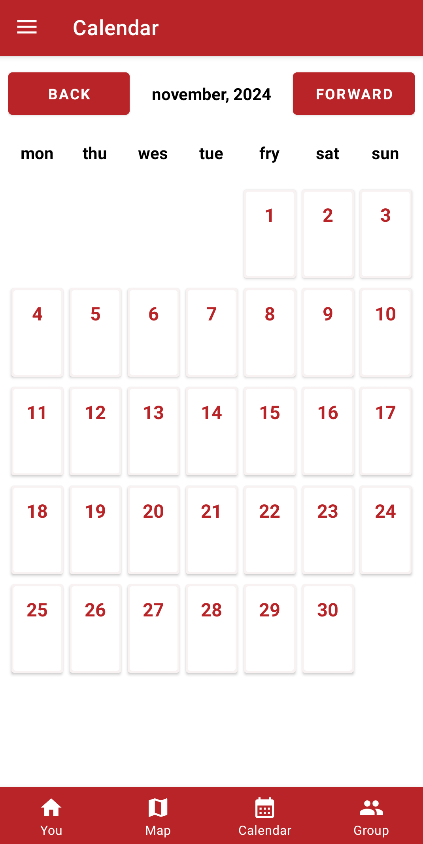
\includegraphics[width=0.35\textwidth]{img7.png}}
            }
            \subfigure[Daily Memo Activity]{
                \fbox{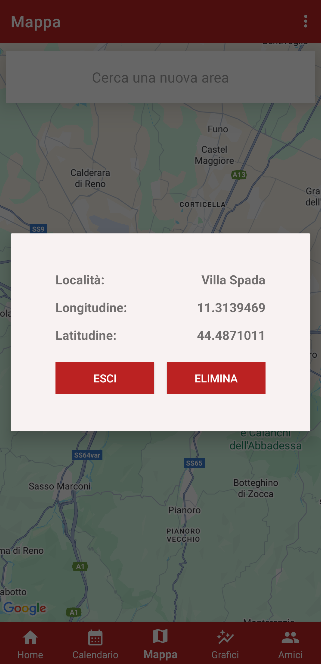
\includegraphics[width=0.35\textwidth]{img8.png}}
            }
        \end{figure}
    \end{center}
    \textbf{Nota bene}: in assenza di una connessione Internet, il \textit{Worker} viene momentaneamente sospeso, rimanendo in attesa di un collegamento, sia Wi-Fi che rete cellulare. \vspace*{7pt}\\
    \textit{Gruppi} \vspace*{7pt}\\
    Tramite l'applicativo è possibile condividere le proprie attività e transizioni con altri \textit{iscritti}, e visualizzare le stesse da loro compiute. Affinchè i dati di un ulteriore utente siano osservabili, occorre che abbia abilitato il \textit{servizio di sincronizzazione}. Tale funzionalità è stata implementata mediante un \textit{Worker}, denominato \textit{SyncBucketWorker}. Si tratta di un \textbf{Worker periodico}, in cui definito un certo arco temporale di attesa, provvede a sincronizzare le informazioni memorizzate localmente rispetto al \textit{dump} contenuto nel \textbf{Bucket} in cloud, agendo in totale autonomia.
    \begin{center}
        \begin{figure}[H]
            \centering
            \subfigure[Group Fragment]{
                \fbox{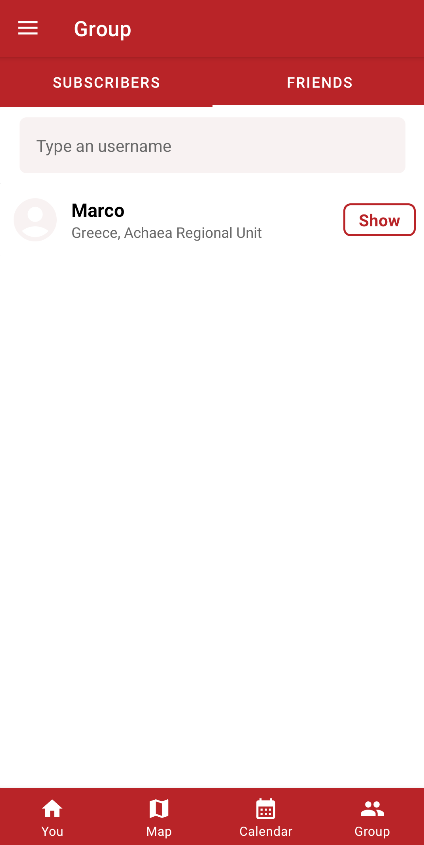
\includegraphics[width=0.35\textwidth]{img9.png}}
            }
            \subfigure[Page Progress User]{
                \fbox{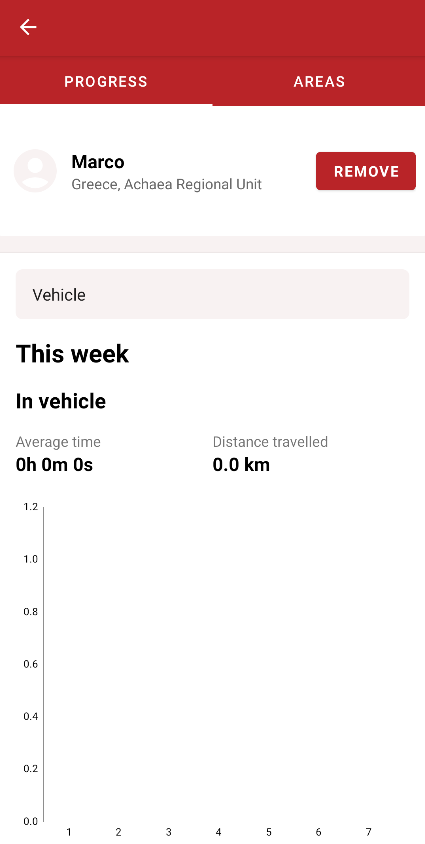
\includegraphics[width=0.35\textwidth]{img10.png}}
            }
        \end{figure}
    \end{center}
    \textbf{Nota bene}: come accade per il \textit{DeleteMemoWorker}, in assenza di connessione il \textit{Worker} descritto viene sospeso. \vspace*{7pt}\\
    \textit{Registrazione attività} \vspace*{7pt}\\
    Come da immagine sottostante, l'utente può registrare quattro tipologie di attività, a cui sono associati alcuni sensori, suddivise in:
    \begin{itemize}
        \renewcommand{\labelitemi}{-}
        \item \textbf{Vehicle Activity}, attività che ricadono nell'utilizzo di un qualche veicolo, in cui è memorizzata la distanza percorsa
        \item \textbf{Run Activity}, attività di corsa, in cui è rilevata la distanza sostenuta e il dislivello affrontato
        \item \textbf{Still Activity}, attività sedentaria, in questo specifico caso non è attuato alcun sensore
        \item \textbf{Walk Activity}, dove è memorizzato il numero di passi e il dislivello affrontato durante la camminata
    \end{itemize}
    \begin{center}
        \begin{figure}[H]
            \centering
            \subfigure[Manual Registration Activity]{
                \fbox{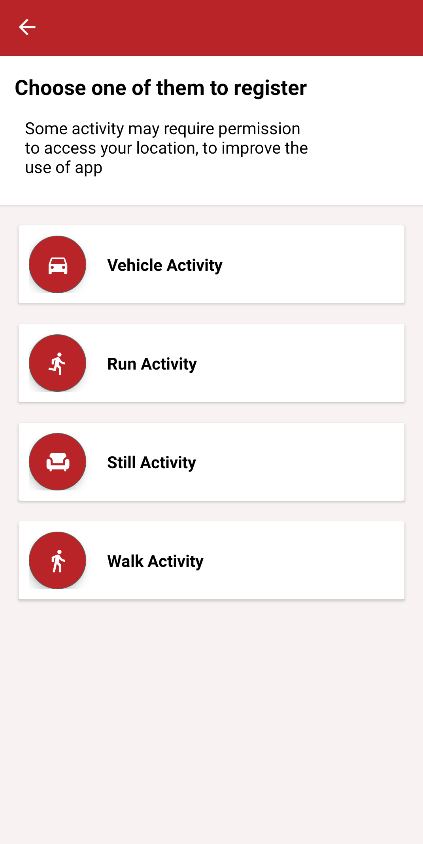
\includegraphics[width=0.35\textwidth]{img11.png}}
            }
            \subfigure[Run Activity]{
                \fbox{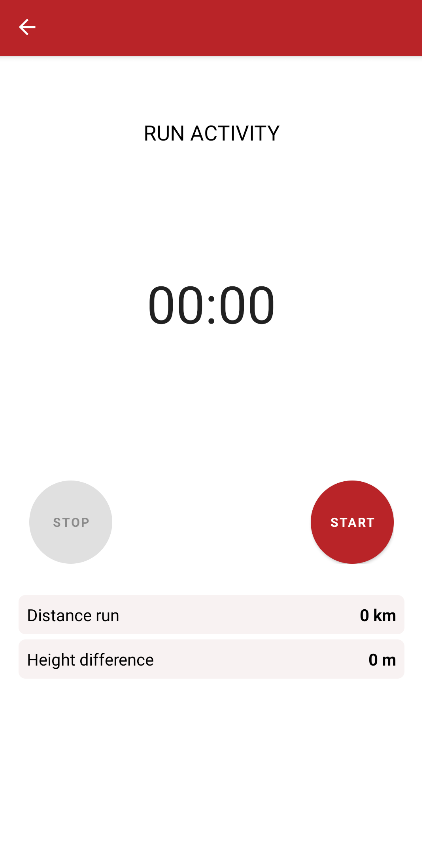
\includegraphics[width=0.35\textwidth]{img12.png}}
            }
        \end{figure}
    \end{center}
    Tutti i dati estrapolati vengono catalogati e salvati all'interno del \textit{Database Locale}, per poi essere successivamente rielaborati per consentirne la corretta
    visualizzazione grafica. Alcuni dei sensori citati, richiedono che l'utente abbia preventivamente accettato il permesso di \textbf{Access Fine Location}, necessario per
    specificare la distanza percorsa durante uno spostamento tramite veicolo oppure durante una corsa.
    Inoltre, sono stati implementati ulteriori due sensori, rispettivamente il \textbf{Step Counter Sensor}, che, come da denominazione, permette di circoscrivere il numero di passi,
    e il \textbf{Sensore di Pressione}, adeguato per indicare il dislivello affrontato durante la rilevazione dell'attività.
    \vspace*{7pt}\\
    \textit{Pannello di controllo} \vspace*{7pt}\\
    Il \textbf{pannello di controllo} costituisce un riferimento univoco in cui l'utente può abilitare oppure disabilitare i servizi disponibili. Al tempo stesso, qualora alcuni di essi non siano mai stati attivati, saranno richiesti i permessi necessari pur di avviare i componenti desiderati. Pertanto, all'interno di tale \textit{Activity} sono richiesti:
    \begin{itemize}
        \renewcommand{\labelitemi}{-}
        \item \textbf{Activity Recognition}, permesso necessario per abilitare il riconoscimento automatico delle attività compiute dall'utente
        \item \textbf{Access Fine Location}, come già narrato, autorizzazione fondamentale per risalire alla geolocalizzazione corrente del dispositivo
        \item \textbf{Access Background Location}, accesso alla geolocalizzazione del dispositivo anche qualora l'applicazione non sia in uso
    \end{itemize}
    Rispettivamente, il primo permesso è necessario per avviare il \textit{service di Activity Recognition}, mentre i restanti sono a loro volta necessari per abilitare
    il \textit{service di Geofencing}.
    \begin{center}
        \begin{figure}[H]
            \centering
            \subfigure[Settings Activity]{
                \fbox{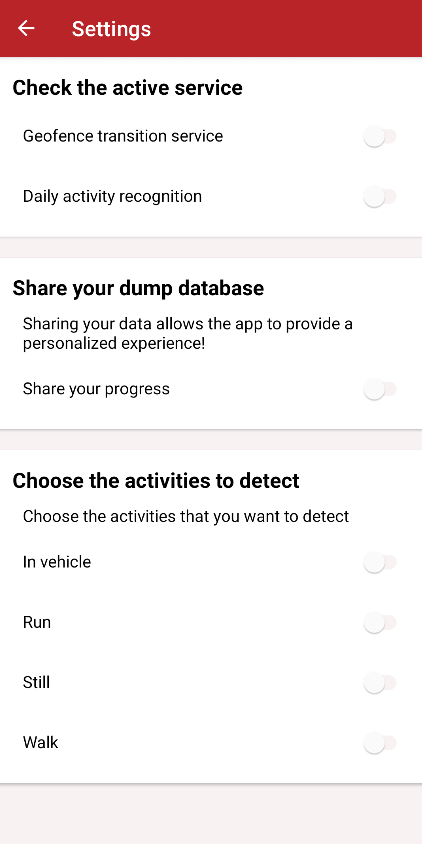
\includegraphics[width=0.35\textwidth]{img13.png}}
            }
        \end{figure}
    \end{center}
    \textbf{Nota bene}: il layout riporta nella sezione finale un breve catalogo di tutte le attività che il servizio è in grado di gestire e manipolare; in assenza di \textit{Toggle} selezionati non sarà possibile avviare il riconoscimento automatico delle attività, anche qualora il \textit{service} sia stato attivato.

    \newpage
    \subsection*{Scelte implementative}
    Nella sezione seguente sono riportate le considerazioni adeguate durante il proseguimento del progetto. L'obiettivo del paragrafo consiste nella definizione e stesura degli aspetti cruciali che abbiano maggiormente inciso durante l'implementazione. \vspace{7pt}\\
    \textit{Model-View-ViewModel} \vspace{7pt}\\
    Come già accennato dall'introduzione, uno dei punti cardine su cui si basa il progetto è il design pattern architetturale \textbf{Model-View-ViewModel}.
    Questo approccio separa la \textit{View}, denominata entità attiva, dal \textit{Model}, contenitore statico di dati, permettendone lo scambio. \\
    Il \textit{ViewModel} è incaricato di mantenere aggiornate le strutture dati che possiedono informazioni del \textit{Model}. Ciò avviene per garantire che tutti i soggetti il cui comportamento può variare in base al contenuto dei dati del \textit{Model}, possano essere notificati dinnanzi ad una qualsiasi variazione.
    Comportamento reso possibile mediante l'impiego di \textbf{LiveData}, a loro volta basati sul concetto di \textit{Observables}.
    \begin{lstlisting}[language=Java]
class NetworkViewModel: ViewModel() {

    private val _currentNetwork = MutableLiveData<Boolean>()
    val currentNetwork: LiveData<Boolean> get() = _currentNetwork

    init {
        _currentNetwork.postValue(MyNetwork.isConnected)
    }

    fun setNetwork(enabled: Boolean) {
        if (_currentNetwork.value != enabled) {
            _currentNetwork.postValue(enabled)
        }
    }
}
    \end{lstlisting}
    Lo snippet di codice precedente, definisce il metodo implementato per aggiornare tutte le componenti dell'applicazione che siano interessate allo stato corrente della connessione. All'interno delle classi è sviluppata una funzione \textit{Observer} dedita ad acquisire i potenziali cambiamenti del \textit{LiveData} circoscritto, abilitanto oppure disabilitando le feature che richiedano una connessione persistente. \vspace{7pt}\\
    \textit{Jetpack Compose} \vspace{7pt}\\
    \textbf{Jetpack Compose} è un framework utilizzato per l'implementazione della \textit{User Interface} di un'applicazione Android.
    Rappresenta uno strumento in grado di accelerare lo sviluppo dell'interfaccia grafica, concentrando in un solo componente,
    \textit{Activity} o \textit{Fragment}, tutto il codice necessario per la sua realizzazione. \vspace{7pt}\\
    Ogni funzione che si accinge a definire qualsiasi \textit{View}, deve riportare la \textit{keyword @Composable}. 
    \begin{lstlisting}[language=Java]
@Composable
private fun DefineFloatingButton(description: String, icon: ImageVector, onClick: () -> Unit) {
    FloatingActionButton(
        onClick = {
            onClick()
        },
        containerColor = colorResource(id = R.color.uni_red),
        elevation = FloatingActionButtonDefaults.elevation(4.dp),
        shape = CircleShape
    ) {
         Icon(
            imageVector = icon,
            contentDescription = description,
            tint = Color.White
        )
    }
}
    \end{lstlisting}
    Il progetto proposto adotta un approccio \textit{ibrido}, ossia impiega i layout realizzati mediante file con estensione \textit{XML} assieme a specifici tag \textit{ComposeView}, articolando i due paradigmi. La scelta di una composizione simile, ha facilitato lo sviluppo di tutti i componenti grafici attesi da un aspetto comportamentale, ovviando a potenziali dipendenze che avrebbero potuto causare differenti problematiche dinnanzi a modifiche necessarie. \vspace{7pt}\\
    \textit{Room} \vspace{7pt}\\
    Per la gestione del \textit{Model} è stato utilizzato \textbf{Room}. La libreria ha permesso di creare e di manipolare con estrema semplicità un \textit{Database Relazionale}, memorizzando al suo interno tutte le informazioni estrapolate durante l'utilizzo dell'applicazione da parte dell'utente. \vspace{7pt}\\
    Dichiarata un'istanza della base di dati, è necessario definire le \textit{Entity}, ossia le tabelle dedotte durante la stesura del \textit{Modello E-R}, e i \textit{DAO}, contenenti tutte le funzioni desiderate. \vspace{7pt}\\
    \textit{AWS} \vspace{7pt}\\
    Per consentire agli utenti di condividere i propri progressi è stato utilizzato \textit{AWS}. La scelta è ricaduta su di esso per le conoscenze pregresse e l'intuitiva implementazione garantita dalla SDK di Kotlin. Abilitato il servizio in questione, presente all'interno del \textit{pannello di controllo}, è programmato un \textbf{Worker periodico}, incaricato di effettuare un \textit{dump} della basi di dati in formato \textit{JSON}, successivamente caricato all'interno di un \textit{bucket} mediante una richiesta \textit{AWS-S3Client}. In questo modo è possibile garantire totale autosufficienza della feature, poichè provvede autonomamente a memorizzare i record del database mediante l'ausilio del servizio esterno. Qualora l'utente decidesse di non condividere più i propri progressi, potrà semplicemente disabilitare la funzionalità dal \textit{pannello di controllo}.
    \vspace{7pt}\\
    \textit{Background operations} \vspace{7pt}\\
    Le operazioni in background sviluppate all'interno del progetto si articolano in tre sezioni differenti, così suddivise:
    \begin{itemize}
        \renewcommand{\labelitemi}{-}
        \item \textbf{Activity Recognition}, deduzione automatica dell'attività fisica conseguita dall'utente. Dopo aver precedentemente stabilito quali attività siano di suo interesse, l'applicazione mediante un \textit{Broadcast Receiver} e un \textit{Service}, dedito alla memorizzazione dei dati estrapolati, provvede a notificare l'utilizzatore
        \item \textbf{Geofencing}, recinti virtuali attuati per contrassegnare località di interesse. A partire dalle coordinate geografiche, è realizzata un'area circolare avente un raggio prestabilito; qualora l'utente dovesse varcare la soglia di una di queste circonferenze, l'applicativo memorizza l'evento all'interno del Database Locale ed invia una notifica al dispositivo 
        \item \textbf{Connectivity}, \textit{Broadcast Receiver} registrato per acquisire tutti i cambiamenti incisivi di connessione che interessino il dispositivo
    \end{itemize}
    A livello implementativo, tutte le \textit{background operations} riportate sono caratterizzate da un'architettura piuttosto simile.
    Ad ognuno di esse è stato associato un \textit{Broadcast Receiver}, responsabile di intercettare gli intenti inviati dal sistema e di risvegliare i \textit{Service} circoscritti. Per attivare i servizi, sono stati implementati dei \textit{Worker}, incaricati di effettuare alcune azioni di \textit{pre-processing} prima di richiamare la funzione \textit{startService()}. Successivamente i \textit{Service}, ottenuti i dati necessari, provvedono a salvare le informazioni dedotte all'interno della base di dati. \vspace{7pt}\\
    Nota a margine per quanto riguarda l'operazione \textit{Connectivity}. Il servizio citato, oltre ad aggiornare lo stato corrente della connessione, permette di variare la dimensione delle \textit{Geofence}. Ciò avviene mediante l'impiego del \textit{Geofence Service};
    una volta risvegliato, si accerta della tipologia di connessione corrente, e varia di conseguenza il perimetro dell'aree di interesse,
    in ottica di risparmio energetico e per garantire maggiore accuratezza.
    \begin{lstlisting}[language=Java]
class ActivityPreprocessingWorker(private val context: Context, workerParams: WorkerParameters): Worker(context, workerParams) {

    override fun doWork(): Result {
        val type = inputData.getInt("TYPE", 4)
        val transition = inputData.getInt("TRANSITION", -1)

        val serviceIntent = Intent(context, ActivityRecognitionService::class.java).apply {
            val items = if (transition == 0) {
                Pair(
                    ActivityRecognitionService.Actions.INSERT.toString(),
                    "ARRIVAL_TIME"
                )
            } else {
                Pair(
                    ActivityRecognitionService.Actions.UPDATE.toString(),
                    "EXIT_TIME"
                )
            }

            action = items.first
            putExtra("ACTIVITY_TYPE", type)
            putExtra(items.second, System.currentTimeMillis())
        }

        context.startService(serviceIntent)

        return Result.success()
    }
}
    \end{lstlisting}
\end{document}